% Options for packages loaded elsewhere
\PassOptionsToPackage{unicode}{hyperref}
\PassOptionsToPackage{hyphens}{url}
\PassOptionsToPackage{dvipsnames,svgnames*,x11names*}{xcolor}
%
\documentclass[
]{article}
\usepackage{amsmath,amssymb}
\usepackage{lmodern}
\usepackage{ifxetex,ifluatex}
\ifnum 0\ifxetex 1\fi\ifluatex 1\fi=0 % if pdftex
  \usepackage[T1]{fontenc}
  \usepackage[utf8]{inputenc}
  \usepackage{textcomp} % provide euro and other symbols
\else % if luatex or xetex
  \usepackage{unicode-math}
  \defaultfontfeatures{Scale=MatchLowercase}
  \defaultfontfeatures[\rmfamily]{Ligatures=TeX,Scale=1}
\fi
% Use upquote if available, for straight quotes in verbatim environments
\IfFileExists{upquote.sty}{\usepackage{upquote}}{}
\IfFileExists{microtype.sty}{% use microtype if available
  \usepackage[]{microtype}
  \UseMicrotypeSet[protrusion]{basicmath} % disable protrusion for tt fonts
}{}
\makeatletter
\@ifundefined{KOMAClassName}{% if non-KOMA class
  \IfFileExists{parskip.sty}{%
    \usepackage{parskip}
  }{% else
    \setlength{\parindent}{0pt}
    \setlength{\parskip}{6pt plus 2pt minus 1pt}}
}{% if KOMA class
  \KOMAoptions{parskip=half}}
\makeatother
\usepackage{xcolor}
\IfFileExists{xurl.sty}{\usepackage{xurl}}{} % add URL line breaks if available
\IfFileExists{bookmark.sty}{\usepackage{bookmark}}{\usepackage{hyperref}}
\hypersetup{
  colorlinks=true,
  linkcolor=blue,
  filecolor=Maroon,
  citecolor=Blue,
  urlcolor=blue,
  pdfcreator={LaTeX via pandoc}}
\urlstyle{same} % disable monospaced font for URLs
\usepackage[margin=1in]{geometry}
\usepackage{color}
\usepackage{fancyvrb}
\newcommand{\VerbBar}{|}
\newcommand{\VERB}{\Verb[commandchars=\\\{\}]}
\DefineVerbatimEnvironment{Highlighting}{Verbatim}{commandchars=\\\{\}}
% Add ',fontsize=\small' for more characters per line
\usepackage{framed}
\definecolor{shadecolor}{RGB}{248,248,248}
\newenvironment{Shaded}{\begin{snugshade}}{\end{snugshade}}
\newcommand{\AlertTok}[1]{\textcolor[rgb]{0.94,0.16,0.16}{#1}}
\newcommand{\AnnotationTok}[1]{\textcolor[rgb]{0.56,0.35,0.01}{\textbf{\textit{#1}}}}
\newcommand{\AttributeTok}[1]{\textcolor[rgb]{0.77,0.63,0.00}{#1}}
\newcommand{\BaseNTok}[1]{\textcolor[rgb]{0.00,0.00,0.81}{#1}}
\newcommand{\BuiltInTok}[1]{#1}
\newcommand{\CharTok}[1]{\textcolor[rgb]{0.31,0.60,0.02}{#1}}
\newcommand{\CommentTok}[1]{\textcolor[rgb]{0.56,0.35,0.01}{\textit{#1}}}
\newcommand{\CommentVarTok}[1]{\textcolor[rgb]{0.56,0.35,0.01}{\textbf{\textit{#1}}}}
\newcommand{\ConstantTok}[1]{\textcolor[rgb]{0.00,0.00,0.00}{#1}}
\newcommand{\ControlFlowTok}[1]{\textcolor[rgb]{0.13,0.29,0.53}{\textbf{#1}}}
\newcommand{\DataTypeTok}[1]{\textcolor[rgb]{0.13,0.29,0.53}{#1}}
\newcommand{\DecValTok}[1]{\textcolor[rgb]{0.00,0.00,0.81}{#1}}
\newcommand{\DocumentationTok}[1]{\textcolor[rgb]{0.56,0.35,0.01}{\textbf{\textit{#1}}}}
\newcommand{\ErrorTok}[1]{\textcolor[rgb]{0.64,0.00,0.00}{\textbf{#1}}}
\newcommand{\ExtensionTok}[1]{#1}
\newcommand{\FloatTok}[1]{\textcolor[rgb]{0.00,0.00,0.81}{#1}}
\newcommand{\FunctionTok}[1]{\textcolor[rgb]{0.00,0.00,0.00}{#1}}
\newcommand{\ImportTok}[1]{#1}
\newcommand{\InformationTok}[1]{\textcolor[rgb]{0.56,0.35,0.01}{\textbf{\textit{#1}}}}
\newcommand{\KeywordTok}[1]{\textcolor[rgb]{0.13,0.29,0.53}{\textbf{#1}}}
\newcommand{\NormalTok}[1]{#1}
\newcommand{\OperatorTok}[1]{\textcolor[rgb]{0.81,0.36,0.00}{\textbf{#1}}}
\newcommand{\OtherTok}[1]{\textcolor[rgb]{0.56,0.35,0.01}{#1}}
\newcommand{\PreprocessorTok}[1]{\textcolor[rgb]{0.56,0.35,0.01}{\textit{#1}}}
\newcommand{\RegionMarkerTok}[1]{#1}
\newcommand{\SpecialCharTok}[1]{\textcolor[rgb]{0.00,0.00,0.00}{#1}}
\newcommand{\SpecialStringTok}[1]{\textcolor[rgb]{0.31,0.60,0.02}{#1}}
\newcommand{\StringTok}[1]{\textcolor[rgb]{0.31,0.60,0.02}{#1}}
\newcommand{\VariableTok}[1]{\textcolor[rgb]{0.00,0.00,0.00}{#1}}
\newcommand{\VerbatimStringTok}[1]{\textcolor[rgb]{0.31,0.60,0.02}{#1}}
\newcommand{\WarningTok}[1]{\textcolor[rgb]{0.56,0.35,0.01}{\textbf{\textit{#1}}}}
\usepackage{longtable,booktabs,array}
\usepackage{calc} % for calculating minipage widths
% Correct order of tables after \paragraph or \subparagraph
\usepackage{etoolbox}
\makeatletter
\patchcmd\longtable{\par}{\if@noskipsec\mbox{}\fi\par}{}{}
\makeatother
% Allow footnotes in longtable head/foot
\IfFileExists{footnotehyper.sty}{\usepackage{footnotehyper}}{\usepackage{footnote}}
\makesavenoteenv{longtable}
\usepackage{graphicx}
\makeatletter
\def\maxwidth{\ifdim\Gin@nat@width>\linewidth\linewidth\else\Gin@nat@width\fi}
\def\maxheight{\ifdim\Gin@nat@height>\textheight\textheight\else\Gin@nat@height\fi}
\makeatother
% Scale images if necessary, so that they will not overflow the page
% margins by default, and it is still possible to overwrite the defaults
% using explicit options in \includegraphics[width, height, ...]{}
\setkeys{Gin}{width=\maxwidth,height=\maxheight,keepaspectratio}
% Set default figure placement to htbp
\makeatletter
\def\fps@figure{htbp}
\makeatother
% Make links footnotes instead of hotlinks:
\DeclareRobustCommand{\href}[2]{#2\footnote{\url{#1}}}
\setlength{\emergencystretch}{3em} % prevent overfull lines
\providecommand{\tightlist}{%
  \setlength{\itemsep}{0pt}\setlength{\parskip}{0pt}}
\setcounter{secnumdepth}{5}
\usepackage{booktabs}
\usepackage{bbm}

% use cleverref package for cross references
% found at https://community.rstudio.com/t/bookdown-equations/38540 
\usepackage[noabbrev]{cleveref}
\renewcommand{\eqref}{\Cref}
\Crefformat{equation}{#2#1#3}
\usepackage{booktabs}
\usepackage{longtable}
\usepackage{array}
\usepackage{multirow}
\usepackage{wrapfig}
\usepackage{float}
\usepackage{colortbl}
\usepackage{pdflscape}
\usepackage{tabu}
\usepackage{threeparttable}
\usepackage{threeparttablex}
\usepackage[normalem]{ulem}
\usepackage{makecell}
\usepackage{xcolor}
\ifluatex
  \usepackage{selnolig}  % disable illegal ligatures
\fi
\newlength{\cslhangindent}
\setlength{\cslhangindent}{1.5em}
\newlength{\csllabelwidth}
\setlength{\csllabelwidth}{3em}
\newenvironment{CSLReferences}[2] % #1 hanging-ident, #2 entry spacing
 {% don't indent paragraphs
  \setlength{\parindent}{0pt}
  % turn on hanging indent if param 1 is 1
  \ifodd #1 \everypar{\setlength{\hangindent}{\cslhangindent}}\ignorespaces\fi
  % set entry spacing
  \ifnum #2 > 0
  \setlength{\parskip}{#2\baselineskip}
  \fi
 }%
 {}
\usepackage{calc}
\newcommand{\CSLBlock}[1]{#1\hfill\break}
\newcommand{\CSLLeftMargin}[1]{\parbox[t]{\csllabelwidth}{#1}}
\newcommand{\CSLRightInline}[1]{\parbox[t]{\linewidth - \csllabelwidth}{#1}\break}
\newcommand{\CSLIndent}[1]{\hspace{\cslhangindent}#1}

\author{}
\date{\vspace{-2.5em}}

\begin{document}

\begin{titlepage}
  \begin{center}
    \vspace*{1cm}
    
    \Huge
    \textbf{Post Processing Covid-19 Forecasts}
    
    \vspace{1.5cm}
    
    Matthias Herp, Joel Beck
    
    \vspace{1.5cm}
    
    \Large
    supervised by
    
    \vspace{0.5cm}
    
    Nikos Bosse
    
    \vspace{2.5cm}
    
    Chair of Statistics, University of G\"ottingen
    
    \vspace{0.5cm}
    
    15.03.2022
            
  \end{center}
\end{titlepage}

\newpage

\renewcommand{\contentsname}{Table of Contents}
\tableofcontents

\newpage


\hypertarget{introduction}{%
\section*{Introduction}\label{introduction}}
\addcontentsline{toc}{section}{Introduction}

\newpage

\hypertarget{analysis-tools}{%
\section{Analysis Tools}\label{analysis-tools}}

Data Analysis is inherently build upon two foundational components: High Quality Data that allows to gain insight into the underlying data generating process and a structured and reproducible way to extract information out of the collected data.

Thus, \Cref{data} introduces the two datasets we worked with whereas \Cref{package} provides an overview about the \texttt{postforecasts} package, a unified framework to apply and analyze various post-processing methods.

\hypertarget{data}{%
\subsection{Data \& Methodology}\label{data}}

This section first introduces the two data sources that all of our analysis is based on.
Afterwards, the final paragraphs explain our evaluation procedure from a theoretical view point.

\hypertarget{uk-covid-19-crowd-forecasting-challenge}{%
\subsubsection{UK Covid-19 Crowd Forecasting Challenge}\label{uk-covid-19-crowd-forecasting-challenge}}

As part of an ongoing research project by the \emph{epiforecasts} group at the London School of Hygiene \& Tropical Medicine the \href{https://www.crowdforecastr.org/2021/05/11/uk-challenge/}{UK Covid-19 Crowd Forecasting Challenge} consisted of submitting weekly predictions of Covid-19 Cases and Deaths in the United Kingdom.
The challenge was not restricted to experienced researchers in the field but rather intended to collect quantile predictions for the upcomning four weeky by non-expert individuals.

One of the main motivations was to gather evidence for or against the hypotheses that humans are highly capable of submitting precise \emph{point forecasts}, yet, at the same time, they tend to be too confident in their beliefs such that prediction \emph{intervals} are chosen too narrow.
In fact, this tendency represents one motivation for post-processing: Extract valuable information from point forecasts and adjust the corresponding prediction intervals with a systematic correction procedure.

In case of individuals that are unfamiliar with statistical methodology specifying forecasts for \(23\) quantiles ranging from 0.01 to 0.99 separately might lead to inconsistencies.
Therefore all participants could determine an uncertainty parameter around their median prediction via an interactive web application such that all quantile predictions could be concluded in an automatic fashion.
Note that this procedure leads to \emph{symmetric} forecast intervals.

The results of the 12-week challenge are \href{https://epiforecasts.io/uk-challenge/}{publicly available}.

\hypertarget{european-covid-19-forecast-hub}{%
\subsubsection{European Covid-19 Forecast Hub}\label{european-covid-19-forecast-hub}}

According to their \href{https://covid19forecasthub.eu/index.html}{webpage} the European Covid-19 Forecast Hub collects \emph{short-term forecasts of Covid-19 cases and deaths across Europe, created by a multitude of infectious disease modelling teams}.

In contrast to the compact UK data described above, the European Forecast Hub data contains almost two million observations for over \(20\) European countries.
Further, the forecasters are knowledgeable research groups that submit their weekly predictions based on statistical models.
Although the data collection continues in regular frequency up to this day, our data set is limited to a \(32\)-week span from March \(2021\) until October \(2021\).

\hypertarget{weighted-interval-score}{%
\subsubsection{Weighted Interval Score}\label{weighted-interval-score}}

In order to quantify if the post-processed prediction intervals improve the original forecasts we chose the \emph{Weighted Interval Score} (WIS) (Bracher et al. 2021) as our evaluation metric.
The WIS is a so-called \emph{Proper Scoring Rule} (Gneiting and Raftery 2007): It incentivizes the forecaster to state their true best belief and cannot be manipulated to its own benefit.
It combines measures for interval \emph{sharpness} as well as \emph{overprediction} and \emph{underprediction} and can thus be understood as a trade-off between prediction \emph{accuracy} and \emph{precision}.

More specifically, for a given quantile level \(\alpha\), true observed value \(y\) as well as lower bound \(l\) and upper bound \(u\) of the corresponding \((1 - \alpha) \cdot 100\)\% prediction interval, the Weighted Interval Score is computed as
\[
\begin{align}
Score_\alpha(y) = (u-l) + \frac{2}{\alpha} \cdot (l-y) \cdot \mathbf{1} (y \leq l) + \frac{2}{\alpha} \cdot (y-u) \cdot \mathbf{1}(y \geq u).
\end{align}
\]
The score of an entire model can then be obtained from a weighted sum over all (included) quantile levels \(\alpha\).

\hypertarget{time-series-cross-validation}{%
\subsubsection{Time Series Cross Validation}\label{time-series-cross-validation}}

Just like any statistical model the post-processing methods must be evaluated on \emph{out-of-sample} data.
Rather than starting from the raw data, i.e.~the observed Covid-19 Cases and Deaths, our data sets already consist of existing quantile predictions.
As a consequence, no part of our data set must be dedicated to fitting the quantile regression models in the first place and our evaluation procedure can be split in two steps:

\begin{enumerate}
\def\labelenumi{\arabic{enumi}.}
\item
  Use a \emph{training set} to learn parameters of the post-processing procedure in consideration.
\item
  Use a \emph{validation set} to evaluate how the learned parameters generalize to unseen data.
\end{enumerate}

Instead of a hard cut-off between the splits we used \emph{Time Series Cross Validation} to leverage a higher fraction of the data set for training.
In contrast to classical cross validation for independent and identically distributed data, time series cross validation iterates through the data set along the time dimension one step at a time.

The process is nicely illustrated in \Cref{fig:ch1-cv}\footnote{Image Source: \url{https://otexts.com/fpp3/tscv.html} (Hyndman and Athanasopoulos 2021).}.

\begin{figure}

{\centering 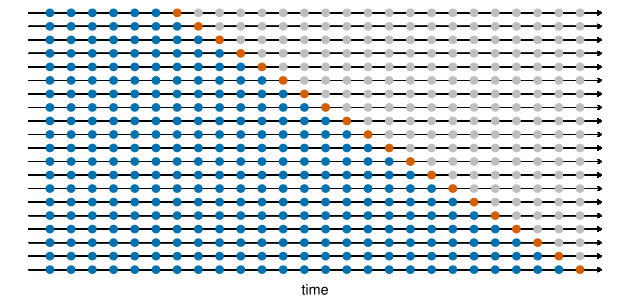
\includegraphics[width=0.8\linewidth]{/Users/maherp/Desktop/Universitaet/Goettingen/3_Semester/Statistisches_Praktikum/post-processing-forecasts/term_paper/images/cv-hyndman} 

}

\caption{Time Series Cross Validation}\label{fig:ch1-cv}
\end{figure}

At each iteration the validation set is composed of the one step ahead prediction based on all observations prior to and including the current time point.
The algorithm typically starts with a minimum number of observations as the initial training set, which can be considered a hyperparameter that has to be specified at the beginning of training.

\hypertarget{package}{%
\subsection{\texorpdfstring{The \texttt{postforecasts} Package}{The postforecasts Package}}\label{package}}

One core aspect of our project was the development of a fully functional R package that unites a collection of different post-processing algorithms into a well-designed and user friendly interface.
This section can be understood as a compact guide how to use our package effectively and explains some of the thought process that went into the implementation.
It is worth noting that the \texttt{postforecasts} package adheres to all formal requirements for an R package such that \texttt{RCMDCHECK} does not produce any warnings or errors.

\hypertarget{overview}{%
\subsubsection{Overview}\label{overview}}

The \texttt{postforecasts} functions that are meant to be visible to the end-user can be grouped into three categories:

\begin{enumerate}
\def\labelenumi{\arabic{enumi}.}
\item
  Exploratory

  The \texttt{plot\_quantiles()}, \texttt{plot\_intervals()} and \texttt{plot\_intervals\_grid()} functions visualize the development of true Covid19 Cases and Deaths over time as well as corresponding original and post-processed quantile predictions.
\item
  Model Fitting

  The \texttt{update\_predictions()} function is the workhorse of the entire \texttt{postforecasts} package.
  It specifies both the raw data and the post-processing method(s) that should be applied to this data set.
  The function returns a list of \(k+1\) equally shaped data frames for \(k\) selected post-processing methods, the first element being the original, possibly filtered, data frame.

  All list elements can be analyzed separately or collectively by stacking them into one large data frame with the \texttt{collect\_predictions()} function.
  The combined data frame is designed to work well with analysis functions that are provided by the \href{https://epiforecasts.io/scoringutils/}{scoringutils package} (Bosse, Sam Abbott, and Gruson 2022).
  Finally, an ensemble model of all selected methods can be appended which will be explained in \Cref{comparison} .
\item
  Evaluation

  As noted in \Cref{data} the Weighted Interval Score is our primary metric to evaluate the \emph{quality} of prediction intervals.
  The \texttt{score()} function of the \texttt{scoringutils} package computes this score for each observation in the data set which can then be aggregated by the related \texttt{summarise\_scores()} function.
  Depending on the \emph{granularity} of the aggregation the output might contain many interval scores of vastly different magnitudes.
  To simplify interpretation the \texttt{eval\_methods()} function computes \emph{relative} or \emph{percentage} changes in the Weighted Interval Score for each selected method compared to the original quantile predictions.
  Further, these relative changes can be conveniently visualized by the \texttt{plot\_eval()} function.
\end{enumerate}

The following section demonstrates the complete workflow described above to give an impression how all these functions interact.

\hypertarget{workflow}{%
\subsubsection{Workflow}\label{workflow}}

We use the Covid-19 data for Germany in \(2021\) that is provided by the European Forecast Hub.

\Cref{fig:ch1-quantiles-germany} illustrates the \(5\)\%, \(20\)\% \(80\)\% and \(95\)\% quantile predictions of the \texttt{EuroCOVIDhub-ensemble} during the summer months of \(2021\) in Germany.

\begin{Shaded}
\begin{Highlighting}[]
\FunctionTok{plot\_quantiles}\NormalTok{(}
\NormalTok{  hub\_germany,}
  \AttributeTok{model =} \StringTok{"EuroCOVIDhub{-}ensemble"}\NormalTok{, }\AttributeTok{quantiles =} \FunctionTok{c}\NormalTok{(}\FloatTok{0.05}\NormalTok{, }\FloatTok{0.2}\NormalTok{, }\FloatTok{0.8}\NormalTok{, }\FloatTok{0.95}\NormalTok{)}
\NormalTok{)}
\end{Highlighting}
\end{Shaded}

\begin{figure}

{\centering \includegraphics[width=1\linewidth]{main_files/figure-latex/ch1-quantiles-germany-1} 

}

\caption{Original Quantile Predictions for Covid-19 Cases and Deaths in Germany 2021}\label{fig:ch1-quantiles-germany}
\end{figure}

The original predictions look quite noisy overall with the clear trend that uncertainty and the interval width increases with growing forecast horizon.
Thus, we want to analyze if one particular post-processing method, \emph{Conformalized Quantile Regression} which is explained in much more detail in \Cref{cqr}, improves the predictive performance for this model on a validation set by computing the Weighted Interval Scores for Covid Cases and Covid Deaths separately.

\begin{Shaded}
\begin{Highlighting}[]
\NormalTok{df\_updated }\OtherTok{\textless{}{-}} \FunctionTok{update\_predictions}\NormalTok{(}
\NormalTok{  hub\_germany,}
  \AttributeTok{methods =} \StringTok{"cqr"}\NormalTok{, }\AttributeTok{models =} \StringTok{"EuroCOVIDhub{-}ensemble"}\NormalTok{, }\AttributeTok{cv\_init\_training =} \FloatTok{0.5}
\NormalTok{)}
\NormalTok{df\_combined }\OtherTok{\textless{}{-}} \FunctionTok{collect\_predictions}\NormalTok{(df\_updated)}
\end{Highlighting}
\end{Shaded}

\begin{Shaded}
\begin{Highlighting}[]
\NormalTok{df\_combined }\SpecialCharTok{|}\ErrorTok{\textgreater{}}
  \FunctionTok{extract\_validation\_set}\NormalTok{() }\SpecialCharTok{|}\ErrorTok{\textgreater{}}
\NormalTok{  scoringutils}\SpecialCharTok{::}\FunctionTok{score}\NormalTok{() }\SpecialCharTok{|}\ErrorTok{\textgreater{}}
\NormalTok{  scoringutils}\SpecialCharTok{::}\FunctionTok{summarise\_scores}\NormalTok{(}\AttributeTok{by =} \FunctionTok{c}\NormalTok{(}\StringTok{"method"}\NormalTok{, }\StringTok{"target\_type"}\NormalTok{))}
\end{Highlighting}
\end{Shaded}

\begin{table}

\caption{\label{tab:ch1-wis-table}Comparison of the Weighted Interval Score after CQR Adjustments}
\centering
\begin{tabular}[t]{cccc}
\toprule
method & target\_type & interval\_score & dispersion\\
\midrule
cqr & Cases & 13.37 & 5.05\\
original & Cases & 13.78 & 3.81\\
cqr & Deaths & 0.05 & 0.01\\
original & Deaths & 0.05 & 0.03\\
\bottomrule
\end{tabular}
\end{table}

\Cref{tab:ch1-wis-table} shows that CQR improved the Weighted Interval Score for Covid Cases on the validation set, whereas the predictive performance for Covid Deaths dropped slightly.

The \texttt{update\_predictions()} and \texttt{collect\_predictions()} combination immediately generalize to multiple post-processing methods.
The only syntax change is a vector input of strings for the \texttt{methods} argument instead of a single string.
Hence, if not desired, the user does not have to worry about which input and output features each method requires in its raw form nor how exactly each method is implemented.
This design allows for maximum syntactic consistency through masking internal functionality.

In the output above CQR increased the \emph{dispersion} of the predictions for Cases significantly.
These wider intervals for specific covariate combinations are visualized in \Cref{fig:ch1-intervals-germany}.

\begin{Shaded}
\begin{Highlighting}[]
\FunctionTok{plot\_intervals}\NormalTok{(df\_combined, }\AttributeTok{target\_type =} \StringTok{"Cases"}\NormalTok{, }\AttributeTok{horizon =} \DecValTok{2}\NormalTok{, }\AttributeTok{quantile =} \FloatTok{0.05}\NormalTok{)}
\end{Highlighting}
\end{Shaded}

\begin{figure}

{\centering \includegraphics[width=1\linewidth]{main_files/figure-latex/ch1-intervals-germany-1} 

}

\caption{Original and CQR-adjusted Prediction Intervals for Covid-19 Cases in Germany}\label{fig:ch1-intervals-germany}
\end{figure}

Indeed, the 2 weeks-ahead \(90\)\% prediction intervals for Cases in Germany are increased by CQR.
The grey dashed line indicates the end of the training set within the time-series cross validation process.

Recall that uncertainty increases with larger horizons.
Similarly, CQR adjustments also increase in size for forecasts that are submitted further in advance, which can be seen in \Cref{fig:ch1-intervalsgrid-germany}.

\begin{Shaded}
\begin{Highlighting}[]
\FunctionTok{plot\_intervals\_grid}\NormalTok{(df\_combined, }\AttributeTok{facet\_by =} \StringTok{"horizon"}\NormalTok{, }\AttributeTok{quantiles =} \FloatTok{0.05}\NormalTok{)}
\end{Highlighting}
\end{Shaded}

\begin{figure}

{\centering \includegraphics[width=1\linewidth]{main_files/figure-latex/ch1-intervalsgrid-germany-1} 

}

\caption{Original and CQR-adjusted Prediction Intervals for different Forecast Horizons}\label{fig:ch1-intervalsgrid-germany}
\end{figure}

Interestingly, CQR expands the intervals only for Cases whereas the forecasts for Deaths are narrowed!

Besides the target type (Cases or Deaths), it is also useful to compare CQR effects across forecast horizons or quantiles.
Quite intuitively, CQR generally has a stronger \emph{relative} benefit for large time horizons and extreme quantiles, where the original forecaster faced a greater uncertainty.
\Cref{fig:ch1-eval-germany} illustrates how, in special cases like this one, the effect on the validation set can show rather mixed trends due to disadvantageous adjustments for the two and three weeks-ahead \(98\)\% prediction intervals.

\begin{Shaded}
\begin{Highlighting}[]
\NormalTok{df\_eval }\OtherTok{\textless{}{-}} \FunctionTok{eval\_methods}\NormalTok{(df\_combined, }\AttributeTok{summarise\_by =} \FunctionTok{c}\NormalTok{(}\StringTok{"quantile"}\NormalTok{, }\StringTok{"horizon"}\NormalTok{))}
\FunctionTok{plot\_eval}\NormalTok{(df\_eval)}
\end{Highlighting}
\end{Shaded}

\begin{figure}

{\centering \includegraphics[width=1\linewidth]{main_files/figure-latex/ch1-eval-germany-1} 

}

\caption{Relative Changes in the WIS through CQR for all Quantile-Horizon combinations}\label{fig:ch1-eval-germany}
\end{figure}

\newpage

\hypertarget{cqr}{%
\section{Conformalized Quantile Regression}\label{cqr}}

\newpage

\hypertarget{qsa}{%
\section{Quantile Spread Adjustment}\label{qsa}}

The general idea behind the Quantile Spread Adjustment (QSA), is to adjust the spreads of each forecasted quantile by some factor. Quantile spreads are defined as the distance between the respective quantile and some basis. As basis three different points in the forecasting spectrum come into question: the median, the next inner neighbor and the symmetric interval quantile. The quantile spread for the different basis are illustrated in \Cref{fig:qs-basis}.

\begin{figure}

{\centering 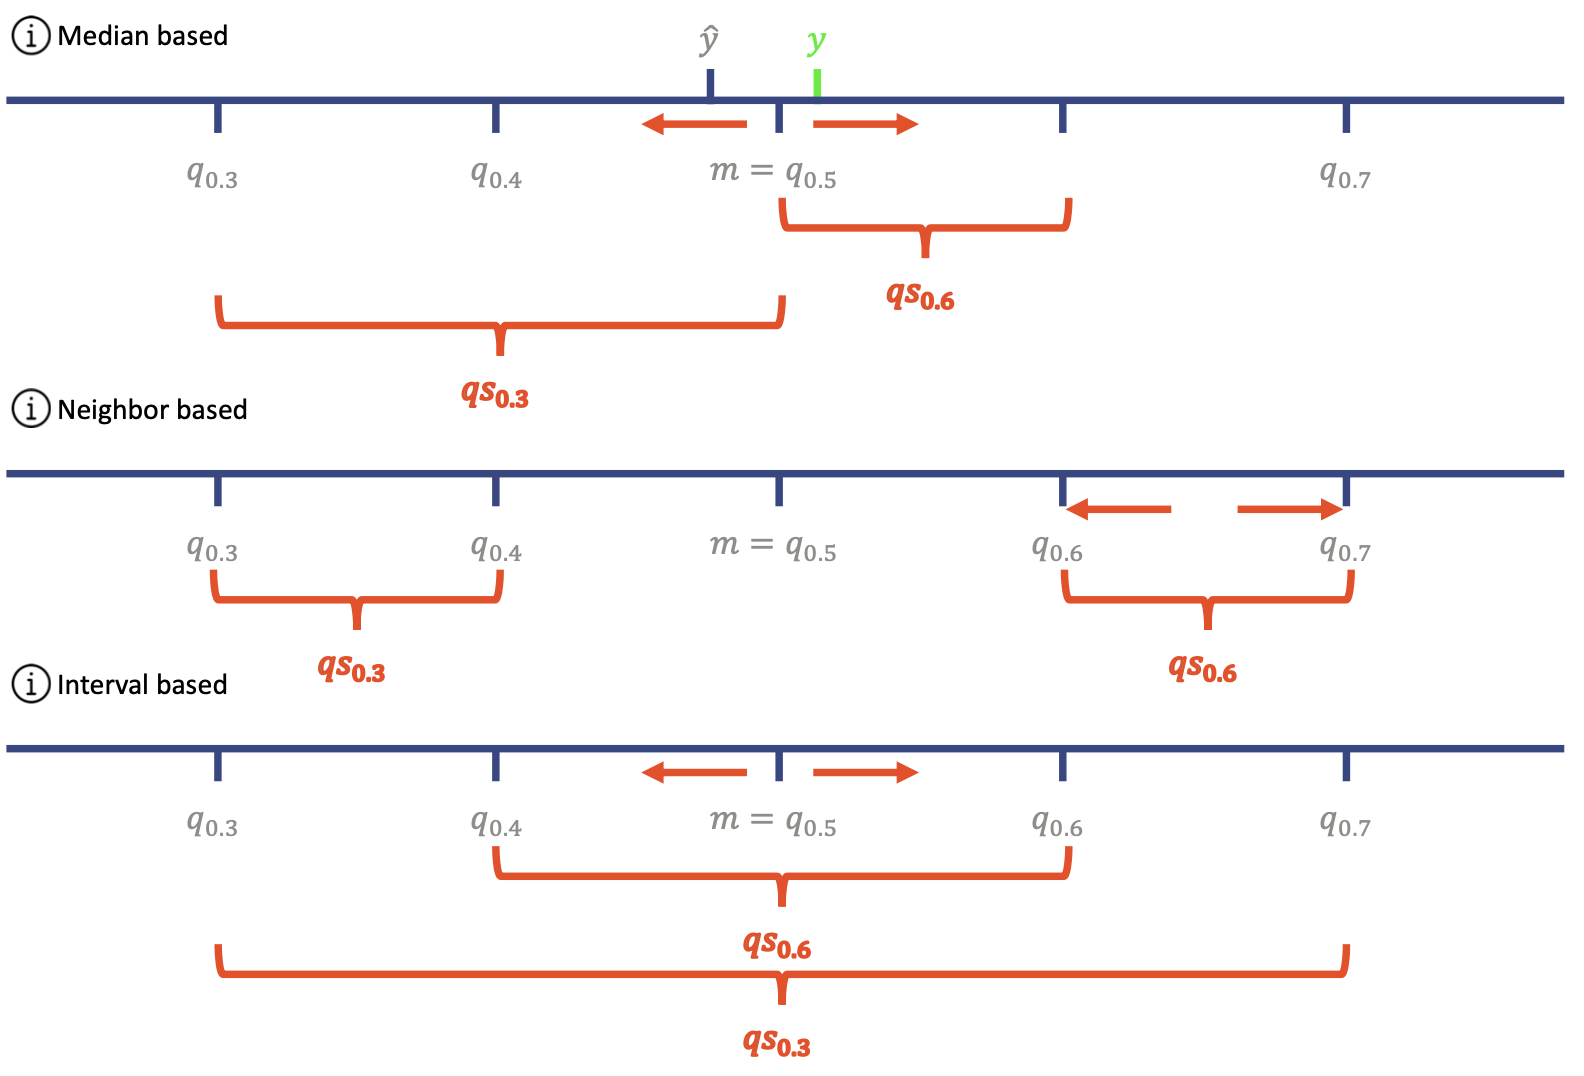
\includegraphics[width=0.8\linewidth]{/Users/maherp/Desktop/Universitaet/Goettingen/3_Semester/Statistisches_Praktikum/post-processing-forecasts/term_paper/images/qs_all} 

}

\caption{Quantile Spreads for different Basis}\label{fig:qs-basis}
\end{figure}

We choose the median based definition of the quantile spreads for two main reasons. First, in contrast to the neighborhood based definition, the median basis has the advantage that different quantile spreads are independent of one another. This property makes finding the optimal quantile spread adjustments for a large set of quantiles much simpler. However it comes at the cost that theoretically adjustments can lead to quantile crossing, which would not be the case for neighborhood based adjustments. Our second reason to use the median basis is that it doesn't restrict adjustments to be symmetric for quantile pairs, as would is the case for the interval based approach.

\hypertarget{theory}{%
\subsection{Theory}\label{theory}}

Using the median based definition, the next step is to determine how to optimally adjust the quantile spreads. As target function, QSA uses the Weighted Interval Score (reference). Equation (reference), with the number of confidence intervals \(p\), the certainty level of a confidence interval \(\alpha_{p}\) and the number of observations \(n\), shows how the QSA weights \(\mathbf{w}\) influence the WIS.

\[
\begin{aligned}
\mathbf{w}^*
&= \operatorname*{arg\,min}_{\mathbf{w} \in \mathbb{R}^p} WIS(\mathbf{y}) \\
&= \operatorname*{arg\,min}_{\mathbf{w} \in \mathbb{R}^p} \sum_{i=1}^p \frac{\alpha_{i}}{2} \sum_{j=1}^n (u_{i,j}^*-l_{i,j}^*) + \frac{2}{\alpha_{i}} \cdot (l_{i,j}^*-y_j) \cdot \mathbf{1} (y_j \leq l_{i,j}^*) + \frac{2}{\alpha_{i}} \cdot (y_j-u_{i,j}^*) \cdot \mathbf{1}(y_j \geq u_{i,j}^*) \\
\text{s.t.} \qquad l_{i,j}^* &= l_{i,j} + (l_{i,j}-m) \cdot (w_i^l-1) \quad \text{and} \quad 
u_{i,j}^* = u_{i,j} + (u_{i,j}-m) \cdot (w_i^u-1)
\end{aligned}
\]

For a given prediction interval level of \(\alpha_{i}\), by varying the QSA factor \(w_i^l\) for the lower and \(w_i^u\) for the upper bound, QSA moves the quantiles from there original values \(l_{i,j}\) and \(u_{i,j}\) to there adjusted values \(l_{i,j}^*\) and \(u_{i,j}^*\). QSA factor values larger than 1 lead to an increase in the prediction interval, thus \(w_i^l > 1\) reduces the value of \(l_{i,j}^*\) and \(w_i^u > 1\) increases the value of\(u_{i,j}^*\). These changes have two effects, on the one side an increase in \(w_i^l\) and \(w_i^u\) reduces the sharpness and increases the WIS, on the other side the increased interval may capture more observation which reduces the under- and overprediction penalities in the WIS. Thus depending on the positions of the observed values and predicted quantiles, QSA will either increase or decrease the interval size in order to minimize the WIS.

The \texttt{postforecasts} package implements the QSA optimization in three, the weight vector \(\mathbf{w}\) restricting, flavors:\texttt{qsa\_uniform}, \texttt{qsa\_flexible\_symmetric} and \texttt{qsa\_flexible}. These are listed in equations (reference).

\[
\begin{aligned}
uniform: w_i = c \quad i \in [0, 1, \ldots, p-1, p], \quad c \in \mathbb{R} \\
flexibel\_symmetric: w_i = w_{p-i} \quad c_{i} \quad i \in [0, 1, \ldots, \frac{p}{2}-1], \quad c_{i} \in \mathbb{R} \\
flexibel: w_i \in \mathbb{R} \\
\end{aligned}
\]
\texttt{qsa\_uniform} restricts all weight vector values to be identical. \texttt{qsa\_flexible\_symmetric} only restricts pair wise adjustments to be identical. It essentially represents unrestricted QSA with interval based adjustments. Finally \texttt{qsa\_flexible} is completely unrestricted as each quantile is adjusted separately.

In addition to different flavors, the \texttt{postforecasts} package also provides the option to regularize the optimization. Equation (reference) depicts the penalization term that is added to the WIS. It is designed to penalize differences between weight vector values by adding a factor proportional to the sum of squared deviation of the weight vector values from there mean. It therefor regularizes towards the \texttt{qsa\_uniform} method and only has an effect for the \texttt{qsa\_flexible\_symmetric} and \texttt{qsa\_flexible} flavors.

\[
\begin{aligned}
\mathbf{w}^*
&= \operatorname*{arg\,min}_{\mathbf{w} \in \mathbb{R}^p} \ WIS_\alpha(\mathbf{y}) + r \cdot Pen(\mathbf{w}), \quad Pen(\mathbf{w}) = \sum_{i=1}^p (w_i - \bar{w})^2 \\
\text{s.t.} \qquad \bar{w} &= \frac{1}{p} \sum_{i=1}^p w_i
\end{aligned}
\]

\hypertarget{optimization}{%
\subsection{Optimization}\label{optimization}}

Underneath the hood, \texttt{postforecasts} accesses the \texttt{optim} function from the R package \href{https://www.rdocumentation.org/packages/stats/versions/3.6.2/topics/optim}{stats} package. From the in \texttt{optim} available optimization methods, \texttt{BFGS} and \texttt{L-BFGS-B} turned out to be the most reliable for QSA. \texttt{BFGS} is named after Broyden, Fletcher, Goldfarb and Shanno and a quasi-Newton method. \texttt{L-BFGS-B}, is a limited memory version of \texttt{BFGS} and additionally also support box constraints. As default value we set the optimization method to \texttt{L-BFGS-B} as it converges faster than \texttt{BFGS} in our data set, due to its limited memory property. The time gain is especially important for the \texttt{qsa\_flexible\_symmetric} and \texttt{qsa\_flexible} methods which take considerably longer than \texttt{qsa\_uniform} for a large number of quantiles. Furthermore \texttt{L-BFGS-B} also has the advantage that we can lower bound the Quantile Spread factor to not drop below zero, hence we can exclude quantile crossing with the median. The optimization method can be accessed in the function \texttt{update\_predictions} functions by setting the \texttt{optim\_method} argument. For \texttt{L-BFGS-B}, the lower and upper bound box constraints can be set with the arguements \texttt{lower\_bound\_optim} and \texttt{upper\_bound\_optim}.
Besides the use of \texttt{optim}, \texttt{postforecasts} also provides a line search optimization which is used by passing \texttt{line\_search}. As the run time increases exponentially with the parameter spaces, this method is currently restricted to the \texttt{qsa\_uniform}. Here, the method runs QSA for all values of the QSA factor within a sequence. This sequence is defined by its upper and lower values set with the arguments \texttt{lower\_bound\_optim} and \texttt{upper\_bound\_optim} as well as its step size set by \texttt{steps\_optim}.
Regarding the QSA optimization functions shape, there is a potential issue: Due to the trade-off between sharpness and coverage defining the WIS, it can happen that an interval of values for the QSA factor result in the same score. This becomes less likelier the more observations and quantiles are available, nevertheless it still has to be kept in mind. The \texttt{line\_search} optimization handles potentially multiple optima by choosing the value closest to 1, hence the smallest possible adjustment of the quantiles. In essence this is a regularization. For the \texttt{BFGS} and \texttt{L-BFGS-B} this simply means that both methods can converge to different optima while attaining the same WIS. In a future version of the package we aim to tackle this by adding a line search after the use of \texttt{BFGS} and \texttt{L-BFGS-B} in order to find the optima closest to 1 and thereby regularize the results..

\newpage

\hypertarget{comparison}{%
\section{Method Comparison}\label{comparison}}

This chapter aims to compare the effectiveness of all Post-Processing methods that were introduced in the previous chapters.
In particular, we investigate if some methods consistently outperform other procedures across a wide range of scenarios, i.e.~different data sets and different covariate combinations.

Further, it will be interesting to observe the \emph{types} of adjustments to the original forecasts:
Some methods might improve the Weighted Interval Score by \emph{extending} the interval width and thus increasing coverage whereas others might yield a similar final score by \emph{shrinking} the prediction intervals leading to a higher precision.
One can imagine even more variants: Moving the interval bounds farther apart or closer together can happen in a \emph{symmetric} or \emph{asymmetric} way and the interval's midpoint might stay \emph{fixed} or get \emph{shifted} throughout the post-processing process.

Before jumping into the analysis, we propose one additional model that in contrast to those we have covered so far, does not add any new information to the equation.
Instead, it \emph{combines} the predictions from existing post-processing methods to build an \emph{ensemble} prediction.
The idea is that leveraging information from multiple independent algorithms can stabilize estimation since the ensemble learns to focus on a model with a strong performance for one particular covariate set while the same model might perform badly for an opposing covariate set and, thus, make little contributions to the ensemble in that case.

Next, we explain the mathematical reasoning behind the ensemble model in more detail.

\hypertarget{ensemble-model}{%
\subsection{Ensemble Model}\label{ensemble-model}}

There exist various options how to combine multiple building blocks into one ensemble.
We chose an approach that can be efficiently computed by well-understood algorithms on the one hand and is highly interpretable on the other hand.
Each quantile prediction of our ensemble model is a \emph{convex combination} of the individual models, i.e.~a linear combination where all weights are contained in the unit interval and sum up to one.
Hence, the resulting value lives on the same scale as the original predictions and each weight can be interpreted as the \emph{fractional contribution} of each building block model.

Consider one particular covariate combination of \textbf{model}, \textbf{location}, \textbf{horizon}, \textbf{target type} and \textbf{quantile}.
Let \(n\) specify the number of observations in the training set within this combination, \(\mathbf{y} \in \mathbb{R}^n\) the vector of true values and \(\hat{\mathbf{y}}_1, \ldots, \hat{\mathbf{y}}_k \in \mathbb{R}^n\) vectors of adjusted predictions from \(k\) different post-processing procedures.

Then, for each such combination, the ensemble model computes weights \(\mathbf{w}^* \in [0, 1]^k\) by solving the following nonlinear constrained optimization problem:
\[
\begin{aligned}
\mathbf{w}^*
= \operatorname*{arg\,min}_{ \mathbf{w} \in [0, 1]^k} WIS_\alpha(\mathbf{y})
&= \operatorname*{arg\,min}_{ \mathbf{w} \in [0, 1]^k} (\mathbf{u}-\mathbf{l}) + \frac{2}{\alpha} \cdot (\mathbf{l}-\mathbf{y}) \cdot \mathbbm{1} (\mathbf{y} \leq \mathbf{l}) + \frac{2}{\alpha} \cdot (\mathbf{y}-\mathbf{u}) \cdot \mathbbm{1}(\mathbf{y} \geq \mathbf{u}), \\
\text{with} \qquad \mathbf{l} &= \sum_{j=1}^{k} w_j \mathbf{l}_j, \;\; \mathbf{u} = \sum_{j=1}^{k} w_j \mathbf{u}_j \\
\text{s.t.} \qquad \sum_{j=1}^{k} w_j &= 1,
\end{aligned}
\]
where all operations for vector inputs \(\mathbf{l}\), \(\mathbf{u}\) and \(\mathbf{y}\) are understood elementwise and the \emph{same} weights \(w_j\), \(j = 1, \ldots, k\) are chosen for lower and upper quantiles.

Hence, we choose the (nonlinear) Weighted Interval Score as our objective function that we minimize subject to linear constraints.
The optimization step is implemented with the \href{https://cran.r-project.org/web/packages/nloptr/index.html}{nloptr} package (Ypma and Johnson 2022), which describes itself as \emph{an R interface to NLopt, a free/open-source library for nonlinear optimization}.

Note that, technically, the weight vector has to be denoted by \(\mathbf{w}_{m, l, h, t, q}^*\) since the computed weights are generally different for each combination.
We omit the subscripts at this point to keep the notation clean.

The Weighted Interval Score always considers \emph{pairs} of quantiles \(\alpha\) and \(1 - \alpha\) that constitute a \((1 - 2 \cdot \alpha)\) prediction interval.
The best results are achieved when a separate weight vector for each quantile pair is computed.
Since our data sets contains \(11\) quantile pairs, \(2\) target types, \(4\) horizons and we consider \(6\) different forecasters, the ensemble model requires solving \(11 \cdot 2 \cdot 4 \cdot 6 = 528\) nonlinear optimization problems for each location, which amounts to \(18 \cdot 528 = 9504\) optimzation problems for the European Hub Data Set.

Due to this high computational cost the \emph{maximum number of iterations} within each optimization was an important hyperparameter that balanced the trade-off between computational feasibilty and sufficient convergence.
Here, we ultimately settled with \(10.000\) maximum steps which could ensure convergence with respect to a \emph{tolerance level} of \(10^{-8}\) in the vast majority of cases.

Finally, it is worth noting that the weight vector of the ensemble model \(\mathbf{w}^*\) is learned on a \emph{training set} such that a fair comparison with all individual post-processing methods on a \emph{validation set} is possible.

\newpage

\hypertarget{conclusion}{%
\section{Conclusion}\label{conclusion}}

\newpage

\hypertarget{appendix-appendix}{%
\appendix}


\hypertarget{first-appendix}{%
\section{First Appendix}\label{first-appendix}}

\hypertarget{second-appendix}{%
\section{Second Appendix}\label{second-appendix}}

\newpage

\hypertarget{references}{%
\section*{References}\label{references}}
\addcontentsline{toc}{section}{References}

\hypertarget{refs}{}
\begin{CSLReferences}{1}{0}
\leavevmode\hypertarget{ref-R-scoringutils}{}%
Bosse, Nikos, Sam Abbott, and Hugo Gruson. 2022. \emph{Scoringutils: Utilities for Scoring and Assessing Predictions}.

\leavevmode\hypertarget{ref-bracher2021}{}%
Bracher, Johannes, Evan L. Ray, Tilmann Gneiting, and Nicholas G. Reich. 2021. {``Evaluating Epidemic Forecasts in an Interval Format.''} \emph{PLOS Computational Biology} 17 (2): e1008618. \url{https://doi.org/10.1371/journal.pcbi.1008618}.

\leavevmode\hypertarget{ref-gneiting2007}{}%
Gneiting, Tilmann, and Adrian E Raftery. 2007. {``Strictly {Proper Scoring Rules}, {Prediction}, and {Estimation}.''} \emph{Journal of the American Statistical Association} 102 (477): 359--78. \url{https://doi.org/10.1198/016214506000001437}.

\leavevmode\hypertarget{ref-hyndman2021}{}%
Hyndman, Rob, and George Athanasopoulos. 2021. \emph{Forecasting: Principles and Practice}. Third. {OTexts}. \url{https://otexts.com/fpp3/}.

\leavevmode\hypertarget{ref-R-nloptr}{}%
Ypma, Jelmer, and Steven G. Johnson. 2022. \emph{Nloptr: R Interface to NLopt}. \url{https://CRAN.R-project.org/package=nloptr}.

\end{CSLReferences}

\end{document}
